\hfill
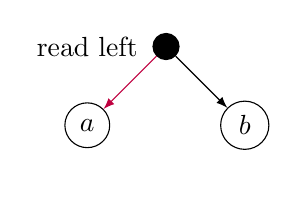
\begin{tikzpicture}
  \node [draw,fill,circle] (r) {};
  \node [draw,circle] (a) [left  of=r, below of=r] {$a$};
  \draw[-latex,color=purple] (r) -- (a);
  \node [draw,circle] (b) [right of=r, below of=r] {$b$};
  \draw[-latex] (r) -- (b);
  \draw[latex-latex,color=white] (a) to [out=-45,in=-135] (b);

  \node () [left of=r] {read left};
\end{tikzpicture}
\hfill
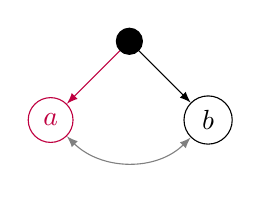
\begin{tikzpicture}
  \node [draw,fill,circle] (r) {};
  \node [draw,color=purple,circle] (a) [left  of=r, below of=r] {$a$};
  \draw[-latex,color=purple] (r) -- (a);
  \node [draw,circle] (b) [right of=r, below of=r] {$b$};
  \draw[-latex] (r) -- (b);
  \draw[latex-latex,color=gray] (a) to [out=-45,in=-135] (b);
\end{tikzpicture}
\hfill
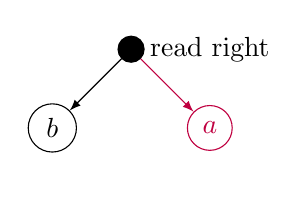
\begin{tikzpicture}
  \node [draw,fill,circle] (r) {};
  \node [draw,color=purple,circle] (a) [right  of=r, below of=r] {$a$};
  \draw[-latex,color=purple] (r) -- (a);
  \node [draw,circle] (b) [left of=r, below of=r] {$b$};
  \draw[-latex] (r) -- (b);
  \draw[latex-latex,color=white] (b) to [out=-45,in=-135] (a);

  \node () [right of=r] {read right};
\end{tikzpicture}
\hfill
